


\chapter{State Of The Art}
\section{Multi Protocol Label Switching (MPLS)}

In MPLS Networks, Packets are forwarded using the 20 Byte Labels unlike the 32 bit IP Address. In order to understand the working of MPLS and its advantages over conventional IP Network, we must understand how the traditional IP traffic processed. 

\subsection{IP Routing}

IP routing\cite{2008} is the process of sending packets from one L3 host to another. The hosts can be in same or different networks and the networks are identified using the IP Addresses. Each packet will have a field for source address and destination address and the packets are forwarded based on the destination address. All the IP Networking devices will maintain a routing table. The devices can be a host machine or a router. The routing table consists of an address field where we can see a 32 bit address and an interface field where we can see a physical or logical interface corresponding to the address. 

\begin{figure}
       \centering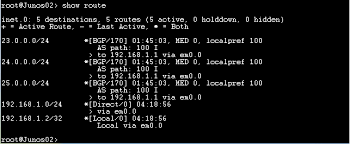
\includegraphics[width=\textwidth]{Final/routing table.png}
       \caption{Sample routing table}
       \label{fig:compbest}
\end{figure}

The figure 1.1 is a sample of routing table from a Juniper router. We can see the networks and the corresponding exit interfaces. Theses routing tables are created and maintained by different routing protocols and each routing protocol have its own mechanisms of finding the best route to the destination. OSPF, RIP and BGP are the well-known routing protocols\cite{2005}.

\subsection{MPLS Switching} 

Multi-protocol label switching (MPLS)\cite{farrel_2004}, is a technique that uses 20-bit labels instead of 32-bit IP Address for sending packet from one MPLS router to another. The Labels are pre populated using different protocols such as Label Distribution Protocol (LDP), Resource Reservation Protocol (RSVP) or Multiprotocol BGP (MP BGP). The packet switching is happening at 2.5 header of the OSI reference model and hence it's called switching. As MPLS need the help of other protocols to create the labels, the name multi-protocol labelled switching  

 \begin{figure}
       \centering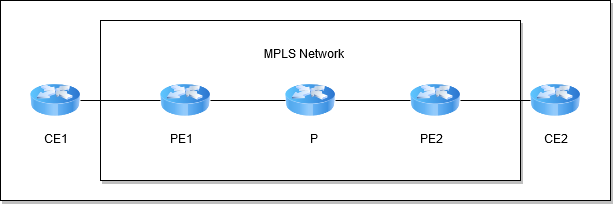
\includegraphics[width=\textwidth]{Final/MPLS Network.png}
       \caption{MPLS Network}
       \label{fig:compbest}
\end{figure}

In the Figure 1.2 the CE1 is a L3 router which operates exclusively on IP address and PE1 is called provider edge router which will operate on both IP address and labels. P is provider router which works exclusively on labels. The incoming packets from CE1 in PE1 taken to a class called Forward equivalence class which assign a label corresponding to the destination IP address. The PE1 then forward the packet to P router which will pop the existing label and add its label corresponding to the destination and finally PE2 will pop the MPLS header from the packet and forward the packet to CE2 using IP routing table. 



 

 \begin{figure}
       \centering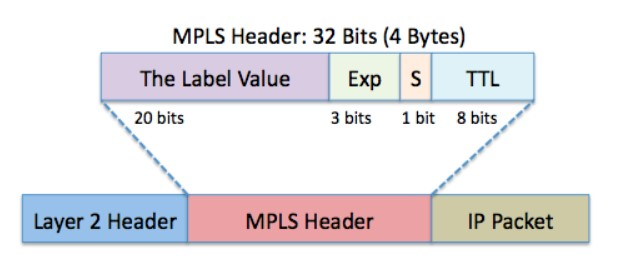
\includegraphics[width=\textwidth]{Final/MPLS Header.jpg}
       \caption{MPLS Header}
       \label{fig:compbest}
\end{figure}


MPLS header gets in between the Ethernet header and the IP Header. The header is 4 bytes in size. The first 20 bits are for the labels, the next 3 bits are for class of service and the next 1 bit for the bottom of stack flag which basically say where the label is positioned. The last 8 bits are for the TTL (time to live). 

\section{Security Requirements in MPLS}

As we know that MPLS is a widely used technology by Service provider to provide VPN Services, the expectation from the VPN Customers and the Service provider is that MPLS Should inherently possess basic security requirements\cite{2010} by its architecture. In this section we can see the basic security requirements of an MPLS Network\cite{davie_farrel_2008}.

\subsection{Address Space Separation}


The expectation is that a packet destined to a host with a particular address in a VPN shouldn't’t reach another VPN or the core. MPLS assume unique address space between 2 non intersecting VPNs and the address space between VPNs should be absolutely independent. This is a basic assumption of address space in MPLS VPNs. In another words the address space in a VPN is very private to it and the same address may can be used in different VPNs for its local connectivity. The routing between 2 VPNs or the VPN and the MPLS core should be independent. Adding a 64-bit RD (Route Distinguisher) by the MPLS core to each IPv4 route will make the VPN unique with the address and unique to the core. The exception is that The IP address of the link between the Provider Edge (PE) and the Customer Edge (CE) router are connected with must be unique. Every PE router is maintaining a VRF table (Virtual Router Forwarding) for each VPNs it connected with. This VRF tables separates the routing between the VPNs. In MPBGP (A signalling protocol), between the core to the other PE routers, the separation is maintained by unique VPN identifiers (VPN ID). This Information is redistributed to all the PE routers and available to all the PEs. So, unless configured to, a packet to host through a VPN cannot reach another VPN.

\subsection{Hiding the MPLS Core from outside}


The Network provider usually hide the internal structure of the MPLS core from outside. In another word, a traceroute should not detail the MPLS Core routers and its addresses. If the internal details of the network are visible to an attacker, its easy to trigger a DOS (Denial-of-service) attack. The network detailing should be hidden even to the VPN Customers and Users. A simple continues ping to any of the PE or P routers in the MPLS core can make the router busy and lead to denial of services.
\subsection{Resistance to attacks}

The Network provider usually hide the internal structure of the MPLS core from outside. In another word. It is easy to trigger a DOS Attack to any exposed resource either by abusing the underlying Routing protocol or by abusing the Signalling protocol (example: attack LDP). This can make instabilities in the Network. 3 Solutions are possible in this case. 1 s isolate the core to the maximum from outside. 2nd is use various packet filters such as ACLs and filter unwanted traffic incoming from outside to the core. 3rd is use the authentication mechanisms provided by the routing protocols and signalling protocols (MD5 Authentication). Out of all these the strongest solution is the isolation of the MPLS Core. The Link connecting the CE and PE should be protected securely.
\subsection{Label spoofing}


As we already discussed that, the packets in MPLS Network is transmitted based on the labels and the PE router maintain an FEC and assign a label to the incoming packet. The design of MPLS is in such a way that the PE cannot accept a pre labelled packet. If an attacker can label an IP packet with a label, the PE cannot accept that, and it can lead to packet drop. So, protecting the packet from the data path of the CE router or even outside is very important. The result of label spoofing within the MPLS core can forward the packet to the convenience of the attacker. Hence protecting the packets from label spoofing Is very important in MPLS.

\section{Possible attacks in MPLS}


MPLS can be attacked in many ways\cite{grayson_guernsey_butts_spainhower_shenoi_2009}. There are tools available which can target various signalling protocols by sending dummy messages to initiate a session, keep the session open or close the session. Loki is one such tool which can use to attack MPLS. It can capture the packets, inject packets, firewall the packets. Let us see some attacks Loki can make in the MPLS Network. In this section, we will attempt to list the different safety assaults that are susceptible to the MPLS network. Security attacks were divided into four kinds: Data Plane Attacks, Control Plane Attacks, MPLS Network Operational and Management Attacks, and Insider Attacks.

\subsection{Attacks on the Data Plane}

Attacks aimed mainly at User or Service Provider data are categorized into data-plane security attacks. These attacks are either aimed at manipulating the data flowing through the MPLS network, removing the data flowing through the MPLS network, injecting malicious data or simply observing maliciously unauthorized data. 

\subsubsection{Taking the MPLS traffic outside the core} 

If an attacker has access to any core device, he can relabel or encapsulate an udp header with a destination address which attacker desired to send. Thus, the attacker can read or access the data from attacker's convenience. In order to do this, the attacker should be aware of the labels used in the traffic. Service providers usually hide the internal architecture of the MPLS core, but still it's not 100 percent safe. 

 
\subsubsection{Modify the Data Traffic}

Manipulating or changing the header fields of the packets can cause severe damage to MPLS Network. This is only possible when the MPLS Internals are exposed to the attacker. Getting the access of the MPLS core is however not easy since service providers usually hide the core from outside. Service providers use firewalls and other filters in their core to filter and block illegitimate packets and accesses. But once the attacker somehow managed to gain the core access, He/ She can make sever damage to the Networks. 

Listed few of the attacks which is possible by packet manipulations, they are: 

\subsubsection{Modify the routes}
 

Attacker can manipulate the network field of the packets the CE router can route the packets to a different destination out of the MPLS Cloud. Attacker can change the L3 field, Labels or encapsulate an UDP Header with completely different Network information. If the attacker gain access to packets part of financial transactions, we can imagine the damage. Rerouting of traffic can take one customers traffic to another customers network. \\

    Path Switching:   Generally, all MPLS packets flow through a Label switched path (LSP) assigned by the service provider. These paths are basically allocated by the service provider based on the labels associated to the packets. Labels are assigned by various parameters such as destination prefix or intended quality of service. For example, if Video streaming packets required a high bandwidth link, then the label will be of the LSP with higher throughput. If an attacker know the particular Label associated to the best LSP, he can label his local traffic such as online gaming traffic and gain best quality of service at the same time the genuine traffic which is expected good quality of service can get dropped. \\
    
    Destination Switching: This can be done in different ways. 1 is by changing the labels , 2nd by changing the destination IP address. Attacker can take the packets to any destination he/she desired and conduct malicious operations. \\
    
    Brute-Force Label Prediction: If an attacker know the destination address, then he/she can inject traffic with some random labels to MPLS networks. Attacker can injects packets by changing labels each time till get a reply from the destination and by doing this the attacker deduce the LSP. Once knew the label information of the LSP, he can use this for malicious operations.\\
    
    
    Address Messages Modification: This is very similar to Label modification. If an attacker gained access to the Customer edge router, he can manipulate the destination address field of the packet and the Provider edge router will take the packet to a Forward Equivalence Class for allocating a label. Suppose the FEC have no information or class for the destination address marked in the packet by attacker, might lead to create a New LSP and send the packets through a compromised link.\\

    Label Edge Router (LER) label Modification:  Customer edge routers are the routers which assign labels to the packets very first time in the MPLS Network and the core routers do the packet forwarding based on the labels PE assigned. If an attacker gained access to the PE router, he can pop the label which PE assigned and push a new label. The Provider router will have to choose an LSP according to the incoming label and if there is no LSP for the incoming label, then this might lead to packet drop or send the packet as IP packet if configured to do so.\\

    VPN label Modification: This attack is very similar to the label modification attack. If an attacker could setup an illegitimate VPNs by using any attacking tools like Loki, then relabelling the packets within the provider edge can cause the P router to switch the packets to the illegitimate VPN. If there is no LSP information in the P router for the new, label then the packet may forward as a plain IP traffic which may be the intention of the attacker. \\
    
    VRF table Modification: This is a very serious attack. A VRF table will have labels and corresponding outgoing physical/logical interfaces. By modifying the VRF table either by changing the labels in the table or the outgoing interface, the attacker can take the packets through the compromised link and to a malicious destination.\\
    
    \subsubsection{Data Insertion attacks}
      

This type of attacks is done by injecting forged traffic into the MPLS network and making the MPLS switch accept it as a genuine traffic and thus making it to forward the packets to the end devices. These packets are sent with malicious intentions to gain certain access to the end device or to read sensitive information. Various Data injection attacks are listed below\\

    Insertion of malicious data traffic to Spoof and Replay: This attack is done by injecting a packet with a spoofed address. The address may belongs to a genuine participant and the MPLS Switch will be assuming the forged packet is from the genuine source. The MPLS switch will reply to the forged spoofed packets. This can cause DOS attack since the MPLS switch is always busy replying the attacker.\\

    Insertion of malicious data using VPN Labels . To do this the attacker should know the labels of the target VPN and the access details of the corresponding egress LER or PER. The attacker inject packets manipulated with the VPN labels and labelled to reach the target LER. Once the packets reach the target LER, it will forward the packets to the target VPN. This attack is not very easy since its need too much of information about the MPLS cloud which is generally very difficult to gain.\\
    
    Insertion of malicious data using LER Labels: This attack is done by manipulating the labels to reach the packets to the target VPN.  The difference between this attack and the one mentioned above is the VPN labels can be ignored. once the packets reach the target LER, then it will forward the packets to an attached VPN site or to a remote VPN site or to the MPLS core. This can even result in looping. To do this attack the attacker should know which LER is accepting packets labelled from outside\\
    
     \subsubsection{Denial-of-Service (DOS) Attacks}
      

DOS is a type of attack which make any service unavailable to its legitimate users. Each system have an upper scale on the number of requests in a second to handle. If the requests coming in are beyond its capacity, then the overloading requests may not be able to serve. If the requests are basically from an attacker just to make the system busy handling the request maximum to its capacity, then the legitimate requests from genuine users won’t be served. Financial services, e commerce websites etc are very vulnerable to such attacks since these types of services expects huge number of transactions in a second. There are many ways an attacker can initiate a DOS attack in MPLS Networks are few of them are listed below.\\

    Modifying the Community Attribute in LERs: To conduct this attack, there should be a target VPN and the attacker should gain access to the PER connected to the VPN. The attacker can modify the VRF table of in the PER associated to the target VPN and then distrust the incoming and outgoing traffic on the target VPN. \\

    Notification Messages Fabrication: This is an attack targeted on LDP Sessions. If the signalling protocol is LDP, then closing the LDP Session will cause tearing down the LSP. If an attacker gets access of an MPLS Link of a MPLS Switch, it can send fabricated LDP Notification message. Upon accepting the LDP Notification message, the LDP Peer will close the LDP Session and the LSP will get closed and traffic through that LSP will be dropped and the Link will be unavailable to the legitimate users. If the attacker gained access of all the links of the MPLS Switch, they can close all the LSPs and causing all the traffic to drop\cite{palmieri_fiore_2007}. \\

    Blocking Keep-Alive Messages:  Similar to the Notification message fabrication, attacker can block the keep alive messages. Not receiving the LDP Keep alive message for a configured interval will lead to closing of the LDP Session and shutting of the LSP. This attack is difficult to identify.\\

    Address Withdraw Messages Fabrication : Address withdraw message is send by LDP when it detect a Link which is down and not in operation. An attacker can send such a manipulated message about one LSR to another causing removal of the link from the received LSRs table. When a genuine packet come to the LSR to a destination originally should be routed through the removed link will get routed through another congested link or will get dropped. This will cause DOS attack to the genuine MPLS users.\\ 

    Label Withdraw Messages Fabrication: Similar to address withdrawal message, attacker can manipulate Label withdrawal message and upon receiving this message the subsequent MPLS router will remove the label from its FEC and lead to flushing of the LSP.\\

    Label Memory Exhaustion: If the LSR is in label retention mode, then flooding those LSRs with label mapping messages will cause it to store such labels. Once the label table memory is exhausted then the LSRs will flush the labels which is in use and use the flooded labels instead. This will cause flushing the working LSPs and creating new LSPs with the manipulated labels.\\

    LSP Deletion: this attack is targeted on RSVP uses, I mean the signalling protocol is RSVP. Similar to label withdrawal message, RSVP can send ‘PathTear’ message if it want to remove any labels from the FEC. Manipulating such packets can cause closing of a working LSP and lead to disruption in the network connectivity and thus DOS attack.\\
    
\subsection{Cross domain attacks}  

A MPLS Customer Edge router(CE) is sending IP (V4 or V6) traffic to Provider Edge(PE) Router and PE router is responsible for assigning labels according to the FEC. An attacker can exploit this cross domain communication between CE and PE (MPLS and Non MPLS domains) and can do various attacks, few are listed below,\\


    Promiscuous Path Acceptance: This attack is possible when the signalling protocol is RSVP. When MPLS traffic engineering is performed, RSVP is used as the signalling protocol as it can perform various quality of service activities. If a service provider MPLS Switch is used for Integrated Services Quality of Service, a Provider Edge Router would receive and accept packets with Router Alert options set by the RSVP as part of QOS and Traffic Engineering. Those packets are guaranteed to be forwarded. This attack is very dangerous because the attacker can do any sort of Traffic Engineering changes in the MPLS Network.\\

    Pre-Labeled Traffic Acceptance: If a Provider Edge (PE) is configured to accept relabelled packets from a Customer Edge Router, then gaining access to a CE router can be dangerous because the attacker can inject packets with relabelled and the MPLS network will be exposed to many kind of signalling attacks.\\
    
\section{Existing security tools}

There are many security tools available to protect MPLS\cite{bănuță_2012} which are external to MPLS. There is no single solution but integrating many of them according to the need will make the MPLS core secure from the attacks discussed above. All the tools have its own limitations and complexities. The tools are different by its mode of operation and provided services. Some of them do payload authentication and some of them do data encryption etc. There is no single tool protects the MPLS core from all the threats discussed above. Based on the threat analysis and understanding the threat and its level of damage, the tools to be used can be determined. Some of the widely used security tools are listed below. 

 
 \subsection{Application Data Encryption}
 
 TLS\cite{rfc8446} is a service used to for reliable secured data transfer. This is very similar to the application data encryption, but TLS create a secure channel between the sender and receiver. There are handshakes and key exchanges in TLS. The payload is send as cipher text. Here also the data encryption and deception is a responsibility of the user application.However the problem with TLS is that the Layer 3 field is plain text and it can be exposed to the attacker. Upon accessing such packet by the attacker, he/she can plan various attacks such as route modification attacks to the data. 
 
\subsection{IP Security (IPSec)}

IPSec\cite{shirazi_asim_irfan_ikram_2010} is another tool which gives the data confidentiality. IPSec can give end to end and hop-by-hop protection. The nest way is to use IPSec between the users seated by an MPLS cloud. I mean between the data source and data destination which is placed either side of the MPLS Network. Data will be encrypted before fed to the MPLS Network. Upon receiving the packet by the destination, IPSec will conduct decryption of data, check the integrity of the data. IPSec can authenticate the participants of the VPN which give additional security. However if the data type Is of non IP, then IPSec cannot be implemented. 

\subsection{Link layer security (MACSec)}

MACSec\cite{jeong_park_park_seo_han_jung_2016} is a tool used to for encrypting at the Ethernet level. MAC sec is hop-by-hop solution which is applied in between two adjacent communications routers. In the case of MPLS, MACsec can be applied between adjacent LSRs. Inorder to gain end to end protection, MAC sec need to be applied between all the LSRs. The drawback of MACsec is that encrypting and decrypting the data at each hope cause additional latency and chances of financial transactions timing out or delay in live streaming etc make MACsec not favourite. \\

      All the above-mentioned tools have its advantages and disadvantages. All the tools are very powerful in doing what it offered at the same time it can lead to additional complexities in the Network. All of the tools are designed for certain use cases. MPLS Opportunistic Security is an additional tool to protect the MPLS Network from the above discussed threats and it's not a substitute or replacement for any of the tools we discussed above. The tools discussed above are not exclusive to MPLS and not desired by evaluating all the MPLS related threats. MPLS OS is designed for MPLS network after analyzing all the possible threats in MPLS Networks. 
 
 
     

 
 
    
    

 


 
